% Preamble
\documentclass[11pt,reqno,oneside,a4paper]{article}
\usepackage[a4paper,includeheadfoot,left=25mm,right=25mm,top=00mm,bottom=20mm,headheight=20mm]{geometry}
%%%% DO NOT EDIT THIS FILE

% Standard packages
\usepackage{amssymb,amsmath,amsthm}
\usepackage{xcolor,graphicx}
\usepackage{verbatim}
\usepackage{mathtools}
\usepackage{hyperref}
% Layout of headers & footers
\usepackage{titling}
\usepackage{fancyhdr}
\newcommand{\runningtitle}{Running Title}
\pagestyle{fancy} \lhead{{\theauthor}} \chead{} \rhead{{\runningtitle}} \lfoot{} \cfoot{\thepage} \rfoot{}

% Hyphenation
\hyphenation{non-zero}

% Theorem definitions in the amsthm standard
\newtheorem{thm}{Theorem}
\newtheorem{lem}[thm]{Lemma}
\newtheorem{sublem}[thm]{Sublemma}
\newtheorem{prop}[thm]{Proposition}
\newtheorem{cor}[thm]{Corollary}
\newtheorem{conc}[thm]{Conclusion}
\newtheorem{conj}[thm]{Conjecture}
\theoremstyle{definition}
\newtheorem{defn}[thm]{Definition}
\newtheorem{cond}[thm]{Condition}
\newtheorem{asm}[thm]{Assumption}
\newtheorem{ntn}[thm]{Notation}
\newtheorem{prob}[thm]{Problem}
\theoremstyle{remark}
\newtheorem{rmk}[thm]{Remark}
\newtheorem{eg}[thm]{Example}
\newtheorem*{hint}{Hint}

%% Mathmode shortcuts
% Number sets
\newcommand{\NN}{\mathbb N}              % The set of naturals
\newcommand{\NNzero}{\NN_0}              % The set of naturals including zero
\newcommand{\NNone}{\NN}                 % The set of naturals excluding zero
\newcommand{\ZZ}{\mathbb Z}              % The set of integers
\newcommand{\QQ}{\mathbb Q}              % The set of rationals
\newcommand{\RR}{\mathbb R}              % The set of reals
\newcommand{\CC}{\mathbb C}              % The set of complex numbers
\newcommand{\KK}{\mathbb K}              % An arbitrary field
% Modern typesetting for the real and imaginary parts of a complex number
\renewcommand{\Re}{\operatorname*{Re}} \renewcommand{\Im}{\operatorname*{Im}}
% Upright d for derivatives
\newcommand{\D}{\ensuremath{\,\mathrm{d}}}
% Upright i for imaginary unit
\newcommand{\ri}{\ensuremath{\mathrm{i}}}
% Upright e for exponentials
\newcommand{\re}{\ensuremath{\mathrm{e}}}
% abbreviation for \lambda
\newcommand{\la}{\ensuremath{\lambda}}
% Make epsilons look more different from the element symbol
\renewcommand{\epsilon}{\varepsilon}
% Always use slanted forms of \leq, \geq
\renewcommand{\geq}{\geqslant}
\renewcommand{\leq}{\leqslant}
% Shorthand for "if and only if" symbol
\newcommand{\Iff}{\ensuremath{\Leftrightarrow}}
% Make bold symbols for vectors
\providecommand{\BVec}[1]{\mathbf{#1}}
% Hyperbolic functions
\providecommand{\sech}{\operatorname{sech}}
\providecommand{\csch}{\operatorname{csch}}
\providecommand{\ctnh}{\operatorname{ctnh}}
% sinc function
\providecommand{\sinc}{\operatorname{sinc}}
% closure of a set
\providecommand{\clos}{\operatorname{clos}}
% The absolute value of a real number or modulus of a complex number, with automatically scaling delimiters
\newcommand{\abs}[1]{\left\lvert#1\right\rvert}
\newcommand{\sgn}{\operatorname{sgn}}

% add two sub and superscripts with a space between them
\newcommand{\Mspacer}{\;} %Spacer for below Matrix display functions
\newcommand{\M}[3]{#1_{#2\Mspacer#3}} %Print a symbol with two subscripts eg a matrix entry
\newcommand{\Msup}[4]{#1_{#2\Mspacer#3}^{#4}} %Print a symbol with two subscripts and a superscript eg a matrix entry
\newcommand{\Msups}[5]{#1_{#2\Mspacer#3}^{#4\Mspacer#5}} %Print a symbol with two subscripts and two superscripts eg a matrix entry
\newcommand{\MAll}[7]{\prescript{#1}{#2}{#3}_{#4\Mspacer#5}^{#6\Mspacer#7}} %Print a symbol with two subscripts and two superscripts eg a matrix entry

% Make really wide hat for Fourier transforms applied to large functions
\usepackage{scalerel}
\usepackage{stackengine}
\stackMath
\newcommand\reallywidecheck[1]{%
\savestack{\tmpbox}{\stretchto{%
  \scaleto{%
    \scalerel*[\widthof{\ensuremath{#1}}]{\kern-.6pt\bigwedge\kern-.6pt}%
    {\rule[-\textheight/2]{1ex}{\textheight}}%WIDTH-LIMITED BIG WEDGE
  }{\textheight}%
}{0.5ex}}%
\stackon[1pt]{#1}{\scalebox{-1}{\tmpbox}}%
}
\providecommand{\widecheck}{\reallywidecheck}

\newcommand\reallywidehat[1]{%
\savestack{\tmpbox}{\stretchto{%
  \scaleto{%
    \scalerel*[\widthof{\ensuremath{#1}}]{\kern-.6pt\bigwedge\kern-.6pt}%
    {\rule[-\textheight/2]{1ex}{\textheight}}%WIDTH-LIMITED BIG WEDGE
  }{\textheight}%
}{0.5ex}}%
\stackon[1pt]{#1}{\tmpbox}%
}


%% Acknowledgements
\newcommand{\AckYNCSRP}[1]{#1 gratefully acknowledges support from Yale-NUS College summer research programme.}
\newcommand{\AckYNCProj}[1]{#1 gratefully acknowledges support from Yale-NUS College project B grant IG18-PRB102.}
\newcommand{\AckYNCWorkshop}[1]{#1 gratefully acknowledges support from Yale-NUS College workshop grant IG18-CW003.}
\newcommand{\AckNICA}[1]{#1 would like to thank the Isaac Newton Institute for Mathematical Sciences for support and hospitality during programme \emph{Complex analysis: techniques, applications and computations}, when work on this paper was undertaken. This work was supported by EPSRC Grant Number EP/R014604/1.}
\newcommand{\AckSMRIIVP}[1]{#1 would like to thank the Sydney Mathematics Research Institute for support and hospitality under the International Visitor Programme.}
 % Standard packages, page layout, theorem environments, macros, etc
% This file contains macros specific to the project.
% You are welcome to add your own macros, but please avoid deleting those written by others.

% Asymptotic notation
\newcommand{\bigoh}{\mathcal{O}}
\newcommand{\lindecayla}{\bigoh\left(\abs{\la}^{-1}\right)}
 % Macros specific to this project.
\usepackage{bbm}
\usepackage{epigraph}
\usepackage{float}
\usepackage{biblatex}
\DeclareMathOperator{\Cech}{\check{C}}
\author{Zhang Liu}
\title{Notes on Topological Data Analysis}
\renewcommand{\runningtitle}{Notes on Topological Data Analysis}
\date{\today}

\begin{document}
\maketitle
\thispagestyle{fancy}

\begin{abstract}
    This document is to serve as a set of notes to fill the gaps in my understanding of Topological Data Analysis relevant to the project. The reference book for this set of notes is \textit{Algebraic Topology} \cite{Hat2002a}, \textit{Topology and Data} \cite{Car2009a}, and \textit{Topology for Computing} \cite{Zom2005a}.
\end{abstract}

% \tableofcontents

\section{Motivation}

First of all, there are four major advantages for using topological methods to deal with point clouds in data analysis.  

\begin{enumerate}
	\item Topology provides qualitative information which is required for data analysis.
	
	\item Metrics are not theoretically justified. Compared to straightforward geometric methods, Topology is less sensitive to the actual choice of metrics. 
	
	\item Studying geometric objects using Topology does not depend on the coordinates. 
	
	\item Functoriality. This is the most important advantage.
	
	\begin{defn}
		For any topological space X, abelian group $A$, and integer $k\geq 0,$ there is assigned a group $H_k(X,A).$
		
		For any $A$ and $k$, and any continuous map $f: X \to Y,$ there is an induced homomorphism $H_k(f,A): H_k(X,A) \to H_k(Y,A).$ Then \textit{functoriality} refers to the following conditions:
		
		\begin{itemize}
			\item  $H_k(f\circ g,A): H_k(f,A) \circ H_k(g,A)$
			\item  $H_k(Id_{X};A) = Id_{H_k(X,A)}.$
		\end{itemize}
	\end{defn}

	Functoriality addresses the ambiguities in statistical clustering methods - in particular the arbitrariness of various threshhold choices. We now illustrate how exactly functoriality could be used in questions related to clustering. 
	
	Let $X$ be the full data set and $X_1,X_2$ are the subsamples from the data set. If the set of clusterings $C(X_1), C(X_2), C(X_1 \cup X_2)$ correspond well (this notion will be defined formally in later section), then we can conclude that the subsample clusterings correspond to clusterings in the full data set $X$. 
\end{enumerate}

\section{Homotopy} \label{sec:homotopy}

\begin{defn}
	\textit{Homotopy} is a family of maps $f_t: X \to Y$ where $t \in I$ such that $F: X\times I \to Y$ defined by $F(x,t) \mapsto f_t(x)$ is continuous.
\end{defn}

\begin{defn}
	Two maps $f_0, f_1$ are \textit{homotopic} if $\exists$ a homotopy $f_t$ between $f_0$ and $f_1$.  
\end{defn}

A special case of homotopy is the deformation retraction. 

\begin{defn}
	A \textit{deformation retraction} of $X$ onto a subspcae $A$ is a homotopy from the identity map of $X$ to a retraction of $X$ onto $A$, $r: X\to X$ such that $r(X) = A$ and $r|_A = \mathbbm{1}$ (or equivalently, retraction is the map $r: X\to X, r^2 =r$). 
\end{defn}

Retraction is the topological analog of projection. To visualize this analogy, we give an example of how some deformation retractions arise from the mapping cylinder.

\begin{defn}
	For a map $f: X\to Y$, the \textit{mapping cylinder} $M_f$ is the quotient space of the disjoint union $(X \times I) \sqcup Y$.
\end{defn}

\begin{defn}
A map $f:X \to Y$ is a homotopy equivalence if there is a map $g: Y \to X$ such that 
\begin{itemize}
	\item $f\circ g$ is homotopic to the identity map on $Y$, and
	\item $g\circ f$ is homotopic to $f$.
\end{itemize}

Two spaces $X,Y$ are\textit{ homotopy equivalent} if there exiss a homotopy equivalence $f: X \to Y. $
\end{defn}

\begin{defn}
	If $f$ and $g$ are homotopic, then $H_k(f,A) = H_k(g,A).$ Then it follows that if $X$ and $Y$ are homotopy equivalent, then $H_k(X,A) \cong H_k(Y,A) $.
\end{defn}

\begin{defn}
	For any field $F$, $H_k(X,F)$ will be a vector space over $F$. Then if $F$ is finite dimensional, its dimension is referred to as the $k$-th Betti number with coefficients in $F$, denoted as $\beta_{k}(X,F).$
	
	The $k$-th Betti number corresponds to an informal notion of the number of independent $k$-dimensional surfaces. If two spaces are homotopy equivalent, then all their Betti numbers are equal. 
	
	Note that the Betti numbers can vary with the choice of the coefficients in $F$. 
\end{defn}

\section{Simplicial Complexes}

\begin{defn}
	An \textit{abstract simplicial complex} is a pair $(V, \Sigma)$, where $V$ is a finite set, and $\Sigma$ is a family of non-empty subsets of $V$ such that 
	$$\sigma \in \Sigma, \tau \subseteq \sigma \implies \tau \in \Sigma.$$
	
	Associated to a simplicial complex is a topological space $|(V,\Sigma)|$. $|(V,\Sigma)|$ may be defined using a bijection $\phi : V \to \{1, 2, \dots,N\}$ as the subspace of $\mathbb{R}^N$ given by the union 
	$$\cup_{\sigma \in \Sigma} c(\sigma),$$
	where $c(\sigma)$ is the convex hull of the set $\{e_{\phi(s)}\}_{s\in \sigma}$, where $e_i$ denotes the $i$th standard basis vector.
\end{defn}

	 We often use abstract simplicial complexes to approximate topological spaces. For simplicial complexes the homology can be computed using only the linear algebra of finitely generated $\mathbb{Z}$-modules. In particular, for simplicial complexes, homology is algorithmically computable (unlike the standard methods for computing the Smith normal form).

\begin{defn}
	Let $X$ be a topological space, and let $\mathcal{U} = \{U_\alpha\}_{\alpha\in A}$ be any covering of $X$. 
	
	The \textit{nerve} of $\mathcal{U}$, denoted by $N\mathcal{U}$, will be the abstract simplicial complex with vertex set $A$, and where a family $\{\alpha_0, \dots, \alpha_k\}$ spans a $k$-simplex if and only if $U_{\alpha_0}\cap U_{\alpha_1} \cap \cdots \cap U_{\alpha_k} \neq \emptyset.$
\end{defn}

One reason that this construction is very useful is the following ``Nerve Theorem." This theorem gives the criteria for $N(\mathcal{U})$ to be homotopy equivalent to the underlying topological space $X$.

\begin{thm}
Suppose that $X$ and $U$ are as above, and suppose that the covering consists of open sets and is numerable. Suppose further that for all $\emptyset \subseteq A,$ we have that $\bigcap_{s\in S} U_s$ is either contractible or empty. Then $N(\mathcal{U})$ is homotopy equivalent to $X$.
\end{thm}

\begin{defn}
	For any subset $V\subseteq X$ for which $X = \bigcup_{v\in V}B_\epsilon(v)$, one can construct the nerve of the covering $\{B_\epsilon(v)\}_{v\in V}$. This construction is referred to as the ``\v{C}ech complex" attached to V and is denoted as $\Cech(V,\epsilon)$.
\end{defn}

\begin{thm}
Let $M$ be a compact Riemannian manifold. Then there is a positive number $e$ so that $\Cech(M, \epsilon)$ is homotopy equivalent to $M$ whenever $\epsilon \leq e$. Moreover, for every $ \epsilon \leq e$, there is a finite subset $V \subseteq M$ so that the subcomplex of $\Cech(V,\epsilon) \subseteq \Cech(M, \epsilon)$ is also homotopy equivalent to $M$.
\end{thm}

However, this construction is computationally expensive. A solution is to construct a simplicial complex which can be recovered solely from the edge information, which motivates the following construction known as the ``Vietoris-Rips complex." 

\begin{defn}
	Let $X$ be a metric space with metric $d$. Then the  \textit{Vietoris-Rips complex} for $X$, attached to the parameter $\epsilon$, denoted by $VR(X,\epsilon)$, will be the simplicial complex whose vertex set is $X$, and where $\{x_0,\dots, x_k\}$ spans a $k$-simplex if and only if $d(x_i,x_j) \leq \epsilon$ for all $0\leq i,j\leq k.$
\end{defn}

\begin{prop}
	Comparing the \v{C}ech complex and the VR compelx:
	$$ \Cech(X,\epsilon) \subseteq VR (X,2\epsilon) \subseteq \Cech(X,2\epsilon).$$
\end{prop}

However, even the VR complex is computationally expensive. A solution, again, is to the Voronoi decomposition which studies the subspaces of Euclidean space. 

\begin{thm}
	Let $X$ be any metric space, and let $\mathcal{L}\subseteq X$ be a subset (called the set of \textit{landmark points}). Given $\lambda \in \mathcal{L}$, we define the \textit{Voronoi cell} associated to $\lambda, V_\lambda$, by
	$$V_\lambda = \{x\in X| d(x,\lambda) \leq d(x,\lambda^\prime)\} \forall \lambda^\prime \in \mathcal{L}.$$
\end{thm}


\begin{defn}
	Similar to how we define the \v{C}ech complex above, we define the Delaunay complex attached to $\mathcal{L}$ to be the nerve of this covering.
\end{defn}

However, for finite metric spaces, the Delaunay complex generically produces degenerate (i.e. discrete) complexes with no $1$-simplices. To solve this, we modify the definition to accommodate pairs of points which are ``almost" equidistant from a pair of landmark points. We thus have the definition below: 
\begin{defn}
	Let X be any metric space, and suppose we are given a finite set $\mathcal{L}$ of points in $X$ (called the landmark set), and a parameter $\epsilon> 0$. For every point $x \in X$, we let $m_x$ denote the distance from this point to the set $\mathcal{L}$, i.e., the minimum distance from $x$ to any point in the landmark set.
	
	Then we define the\textit{strong witness complex} attached to this data to be the complex $W^s(X,\mathcal{L}, \epsilon)$ whose vertex set is $\mathcal{L}$, and where a collection $\{l_0, \dots, l_k\}$ spans a $k$-simplex if and only if there is a point $x \in X$ (the witness) so that $d(x, l_i)\leq m_x + \epsilon$ for all $i$. 
	
	We can also consider the version of this complex in which the $1$-simplices are identical to those of $W(X,\mathcal{L},\epsilon)$, but where the family $\{l_0, \dots, l_k\}$ spans a $k$-simplex if and only if all the pairs $(l_i, l_j)$ are $1$-simplices. We will denote this by $W^s_{VR}$.
\end{defn}

A modified version of the strong witness complex is also useful:

\begin{defn}
	We construct the\textit{weak witness complex}, $W^w(X,\mathcal{L}, \epsilon)$, attached to the given data by declaring that a family $\Lambda = \{l_0, \dots, l_k\}$ spans a $k$-simplex if and only if $\Lambda$ and all its faces admit $\epsilon$ weak witnesses. 
	
	Similar to the definition for strong witness complex, we can also consider the version of the weak witness complex in which the $1$-simplices are identical to those of $W(X,\mathcal{L},\epsilon)$, but where the family $\{l_0, \dots, l_k\}$ spans a $k$-simplex if and only if all the pairs $(l_i, l_j)$ are $1$-simplices. We will denote this by $W^w_{VR}$.
\end{defn}

\section{Category Theory Pre-requisites}
\epigraph{It frames a possible template for any
mathematical theory: the theory should have
nouns and verbs, i.e., objects, and morphisms,
and there should be an explicit notion of
composition related to the morphisms; the theory
should, in brief, be packaged by a category.}
{Barry Mazur, ``When is one thing equal to some
other thing?”}

\begin{defn}
	A \textit{category} consists of
	\begin{itemize}
		\item a collection of objects $X,Y,Z,\dots$
		\item a collection of morphisms $f,g,h,\dots$
	\end{itemize}
	so that:
	\begin{itemize}
		\item Each morphism has specified domain and codomain objects; the notation $f : X \to Y$
		signifies that $ f$ is a morphism with domain $X$ and codomain $Y$.
		\item Each object has a designated identity morphism $\mathbbm{1}_X : X \to X$.
		\item For any pair of morphisms $f,g$ with the codomain of $f$ equal to the domain of $g$, there exists a specified composite morphism $gf$ whose domain is equal to the domain of
		$f$ and whose codomain is equal to the codomain of $g$, i.e.,:
		$$f : X \to Y, g: Y \to Z \rightsquigarrow  g f : X \to Z .$$
	\end{itemize}
\end{defn}

A natural question to ask is: what is a morphism between categories? This leads to the definition of a functor:
\begin{defn}
	A \textit{functor} $F : C \to D$, between categories $C$ and $D$, consists of the following data:
	\begin{itemize}
		\item An object $F_c \in D$, for each object $c \in C$.
		\item A morphism $F f : Fc \to Fc^\prime \in D$, for each morphism $f : c \to c^\prime \in C$, so that the	domain and codomain of $F f$ are, respectively, equal to $F$ applied to the domain or codomain of $f$.
	\end{itemize}

	The assignments are required to satisfy the following two functoriality axioms:
	\begin{itemize}
		\item For any composable pair $f, g in C$,$Fg \cdot F f = F(g \cdot f).$
		\item For each object $c$ in $C$, $F(\mathbbm{1}_c) = \mathbbm{1}_{Fc}.$
	\end{itemize}

	Put concisely, a functor consists of 
	
	\begin{enumerate}
		\item a mapping on objects and 
		\item a mapping on morphisms that preserves all of the structure of a category, namely domains and codomains,	composition, and identities.
	\end{enumerate}
\end{defn}

As already mentioned in Section 1, functoriality plays a key role in topological data analysis.  

\cite{}

\begin{defn}
	Let $A$ be a ring. A \textit{left module} $M$ over $A$ consists of an abelian group (also denoted $M$) and a law of composition $A \times M \to M$ (denoted $(a, x) \mapsto ax)$ such that
	
	\begin{align}
	a(bx)=(ab)x &\text{ for }a, b \in A, x \in M, \\
	1x = x &\text{ for } x \in M,\\
	(a + b)x = ax + bx &\text{ for } a, b \in A, x \in M,\\
	a(x + y) = ax + ay &\text{for } a \in A, x, y \in M.
	\end{align}

	(4) asserts that $\rho(a) : M \to M $defined by $\rho(a)(x) = ax$ is an endomorphism of the	underlying abelian group of the module, while the first three statements assert that $\rho : A \to End(M)$
	is a ring homomorphism. Conversely, given such a homomorphism, we may define a module structure on $M$
	by setting $ax = \rho(a)(x)$.
	
	Analogically, we can define the right module over $A$.
\end{defn}

Note that the concept of module is a generalization of the concept of vector space. The condition that ``a vector space is finite dimensional” generalizes to the condition that ``a module is finitely generated”. A basis of a module is a generating set that is linearly independent over the ring. Unfortunately, such sets rarely exist: only free modules have bases. Usually, we have to consider a (minimal) system of generators instead of a basis.

\begin{defn}
 A ring R is called \textit{graded} (or more precisely, $\mathbb{Z}$-graded ) if there exists a	family of subgroups ${Rn}_{n\in \mathbb{Z}}$ of $R$ such that
 \begin{enumerate}
 	\item $R = \oplus_n R_n$ (as abelian groups), and
 	\item $R_n \cdot R_m \subseteq R_{n+m} \forall n, m.$
 \end{enumerate}
\end{defn}

\begin{defn}
	Let $R$ be a graded ring and $M$ an $R$-module. We say that $M$ is a\textit{ graded
	$R$-module} (or has an $R$-grading) if there ${M_n}{n\in \mathbb{Z}} $ of $M$ such	that

\begin{enumerate}
	\item $M = \oplus_n M_n$ (as abelian groups), and
	\item $R_n \cdot M_m \subseteq M_{n+m} \forall n, m.$
\end{enumerate}

	If $u \in M \setminus \{0\}$ and $u = u_{i_1} + \cdots + u{i_k} $ where $u_{i_j}\in R_{i_j}\setminus \{0\}$, then $u_{i_1}	, \dots, u{i_k}$ 
	are called\textit{ the homogeneous components } of $u$. 
\end{defn}

\section{Persistence}

The main idea of \textit{persistence} is that instead of selecting a fixed value of the threshhold $\epsilon$, we would like to obtain a useful summary of the homological information for all the different values of $\epsilon$ at once. 

\begin{defn}
	Let $\underline{C}$ be any category, and $\mathcal{P}$ a partially ordered set. We regard $\mathcal{P}$
	as a category $\underline{\mathcal{P}}$ in the usual way, i.e. with object set $\mathcal{P}$, and with a unique morphism	from $x$ to $y$ whenever $x \leq y$. Then by a $\mathcal{P}$-persistence object in $C$ we mean a functor
	$\phi : \mathcal{P} \to C$.
	
	 More concretely, it means a family $\{c_x\}{x\in \mathcal{P}} $of objects of $C$ together with morphisms $\phi: xy : cx \to cy$ whenever$ x \leq y$, such that $\phi_{yz} \circ \phi_{xy} = \phi_{xz}$ whenever $x \leq y \leq z$. Note that the $\mathcal{P}$-persistence objects in $C$ form a category in their own	right, where a morphism $F$ from $\phi$ to $\Phi$ is a natural transformation. Again, in
	more concrete terms, a morphism from a family $\{c_x, \phi_{xy}\}$ to a family $\{d_x, \Phi_{xy}\}$ is a family of morphisms $\{f_x\}$, with $f_x : c_x \to d_x$, and where the diagrams commute:
	\begin{figure}[H]
		\centering
		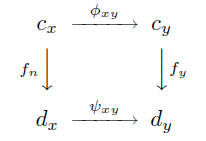
\includegraphics[width=0.3\linewidth]{figures/tda5-1.png}
		\label{fig:tda5-1}
	\end{figure}
\end{defn}

Although we do not have a classification theorem for $\mathbb{R}$-persistence abelian groups, which would then provide a summary of the behavior of the homology of all the complexes $\Cech(X,\epsilon)$, we do have a classification theorem for a subcategory of the category of $\mathbb{N}$-persistence $F$-vector spaces, where $F$ is a field. 

From the $\mathbb{R}$-persistence simplicial complexes, we just need any partial order preserving map $\mathbb{N} \to \mathbb{R}$ to obtain an $\mathbb{N}-$persistence simplicial complex. Then we can use the classification theorem. 

There are at least two useful ways to construct such maps. 

The summary of the methodology is as follows:
\begin{enumerate}
	\item Construct the $\mathbb{R}$-persistence simplicial complex using Cech, Vietoris-
	Rips, or witness methods. We will denote it by $\phi$.
	\item Select a partial order preserving map $f: \mathbb{N} \to \mathbb{R}$.
	\item Construct the associated N-persistence simplicial complex.
	\item Construct the associated N-persistence chain complex with coefficients
	in F. (It is evident from the finiteness hypotheses on X and
	the nature of the constructions that the associated N-persistence F-vector
	spaces are tame.)
	\item Compute the barcodes associated to the N-persistence F-vector spaces
\end{enumerate}

\end{document}
